\section{Big Data Science}

Big Data is much in the news these days, from reports of massive data
dredging by the NSA to tens of millions of credit cards stolen by
hackers from commercial databases.
Big Data has become crucial to scientific advances from understanding the
genome to predicting climate change.
Unfortunately, computer scientists in the workforce are woefully
unequipped for this shifting paradigm.
Indeed, a report by MGI and McKinsey's Business Technology Offices
declares that ``by 2018, the United States alone could face a
shortage of 140,000 to 190,000 people with deep analytical skills as
well as 1.5 million managers and analysts with the know-how to use the
analysis of Big Data to make effective decisions.''\cite{McKinsey}
There are many obstacles to effectively educating students on Big
Data.
Its representation, manipulation, and expression is
challenging, with modern curriculums and programming tools being
inadequate.

\begin{wrapfigure}{r}{0.5\textwidth}
    \begin{center}
		    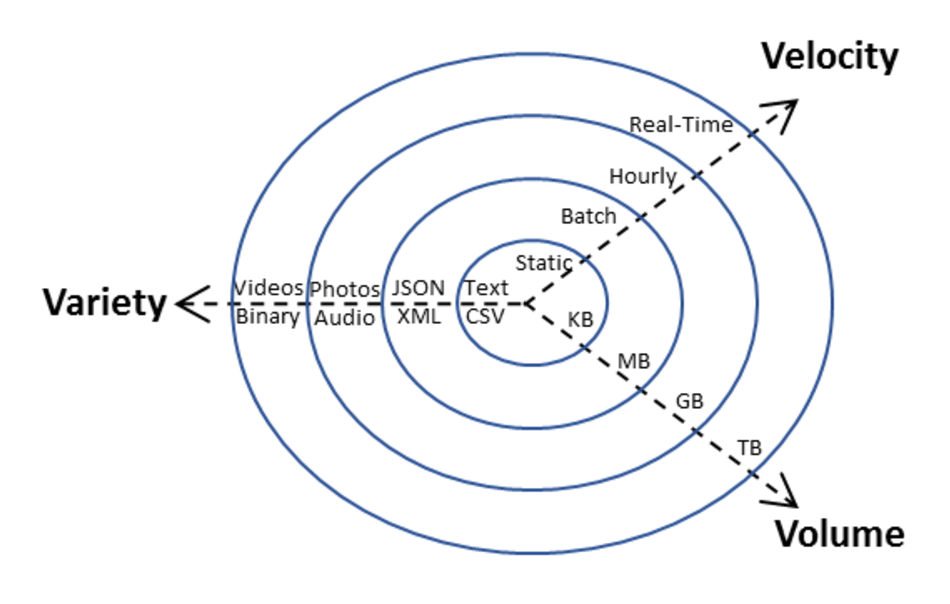
\psfig{file=images/3v-model.eps, width=\linewidth}
    \end{center}
    \vspace{-\bigskipamount}
    \caption{The 3V Model of Big Data}
    \label{fig-3v}
\end{wrapfigure}

Big data has been loosely described as quantities of information that cannot be handled with traditional methods ~\cite{McKinsey}.
But ``traditional methods'' is a vague phrase that has different meanings to different learners. To a Humanities major in their first CS-0 course, the traditional method to sum a list is to use Excel. In this scenario, ``big data'' means anything that won't comfortably fit into Excel's working memory.
However, to a third-year Computer Science major, the traditional method would be to write an iterative or recursive sequential loop; being given big data forces them to explore parallel models of execution.
Clearly, ``bigness'' is a function of the learner's experience, but that is still not a solid definition.

A more precise definition is the ``3V Model'' \cite{douglas2012importance}, which posits that there are three dimensions that distinguish big data from ordinary, run-of-the-mill data:

\begin{description}
	\item[Volume:] The total quantity of the information, usually measured in bytes or number of records. However, this also extends laterally: the number of fields in the structure of the data also impacts the complexity and size. The threshold at which data becomes big is a function of the hardware and software being used -- for instance, embedded systems may consider gigabyte-sized files to be big, while modern servers might not struggle until the petabyte level.
	\item[Velocity:] The rate at which new information is added to the system. High velocity big data implies a distributed architecture, since new data must be arriving from somewhere. The dynamicity of data can vary widely across these architectures, with data updating every year, every day, or even multiple times a second.
	\item[Variety:] The format or formats of the data. Ideally, data are always distributed in a way that is readily accessible -- for instance, simple text-based formats such as CSV and JSON are widely supported, relatively lightweight, and human-readable. More sophisticated data formats for image and audio are also typically well-supported, although still more complicated. However, projects using specialized, compressed binary formats or, more dangerously, multiple formats (e.g., image archives organized with XML files), are more complex.
\end{description}

In the remainder of this section, I describe common challenges associated with different kinds of data.

\subsection{High Velocity Data}

It is not trivial to enable introductory students to work with high velocity data, which is necessarily distributed. Without any scaffolding, it is necessary to delay the use of such data until much later in the course. In a prior paper \cite{realtimeweb-splashe}, we outline the biggest barriers to high velocity data as a context:
\begin{description}
  \item[Access] The process of programmatically downloading and parsing a web-based resource is a non-trivial procedure requiring an understanding of both basic concepts (e.g., function calls, data transformation) and specialized web technology (e.g., the difference between GET and POST calls, building query parameters).
	\item[Non-Idempotency] Because high velocity data is constantly changing, repeated calls to the same URL endpoint can return wildly different results, even over the course of a few minutes. This makes finding errors and testing considerably harder.
	\item[Consistency] Web-based APIs are controlled and developed by independent entities, which means that changes can occur at any time with little to no notification or time for reaction. This means that students' code can become out of date even during the middle of testing their final project.
	\item[Connectivity] Although internet speeds for students on a university campus are typically stable, this does not extend to off-campus students or students that are traveling. If the internet connection is down, then students might be completely unable to make progress.
	\item[Efficiency] Even when the internet connection is stable, it might not always be fast. Requiring a round-trip to a server can greatly drag on the testing and development process, frustrating the student and decreasing the time spent learning.
\end{description}

\subsection{High Volume Data}

In this section, we highlight some of the more challenging aspects of introducing high volume data, similar to how we previously outlined the challenges of high velocity data.
Some of these challenges are technical in nature, and some of them of a more pedagogical nature.
These challenges lead to certain design requirements that must be satisfied in any scaffolding intended to introduce high volume data.

\begin{description}
	\item[Data Transmission:] Internet connections can be difficult and inconsistent, especially for off-campus
and non-traditional students. Although most modern universities boast impressive wired connection
speeds, these speeds rarely extend off-campus. And even when internet connections are top-notch,
they can still be inadequate to serving the needs of transmitting big data collections to an entire
classroom of students. Some affordances must be made to make the data readily available to students without taxing their hard drives unnecessarily.
	\item[Different Contexts and Problems]: Additionally, high volume data offers different contexts and problems than high velocity data.
For instance, high velocity data typically lends itself to small quantities of data that are relevant to the current state of the real world -- for instance, students can walk outside and feel the current weather, which should correlate to real-time weather reports made available by a weather library.
High volume data, on the other hand, lends itself to large quantities of mostly static data -- for instance, crime reports for a long period of time.
Although high velocity data gives authentic answers in the here and now, high volume data gives authentic answers for the future, through trends.
Some fields have both kinds of data available -- meteorologists generate forecasts (high velocity, low volume) by studying historical climate data (high volume, low velocity).
But some fields are not amenable to both -- digital historians typically have large stores of historical information (high volume), but it does not change quickly (low velocity).
Careful consideration must be made when choosing problems and designing contexts so that the data leads to optimally authentic learning experiences.
\end{description}


\subsection{High Variety Data}

\begin{description}
\item[Inconsistency of Storage:] High variety data is composed of many different kinds of file formats -- some of which are more complicated than others.
\item[Inconsistency of Tools:] Different languages usually offer many different tools to interact with the exotic formats of the data -- however, these tools vary greatly in availability, usabililty, and compatability across platforms. For instance, binary image data is supported as a first-class programming object in the Racket programming environment, but can only be loaded using libraries such as Pygame in Python, which the user may or may not have installed.
\end{description}

\subsection{General Challenges of Data}

\begin{description}
	\item[Ensuring Wide Availability:] There is no universal agreement within the Computer Science Education community
on the perfect introductory language \cite{CS2013}. Indeed, individual instructor’s answers will change
depending on what CS course (e.g., CS-0 vs. CS-2) is being considered. Python and Racket/Scheme are growing in
popularity for CS-0/1, but Java is still a dominant choice for both CS-1 and CS-2 [8]. One of the great
successes of the RealTimeWeb project that we are building off was the availability of every API in at
least three common languages (Racket, Python, and Java). In order to ensure wide-spread adoption, our
new infrastructure must also be available in a number of commonly-used languages.
\item[Intentionally secured data] Organizations such as FERPA and HIPPA exist in order to ensure the privacy and dignity of captive populations (e.g., school children, patients). These organizations define rules for how data on such populations can be published and made available. Often, interesting data exists behind walled gardnes. Although novel techniques such as Differential Privacy (where data is probabilistically modified to protect anonymity) can be used to mitigate these problems, it is simply a fact that some data is utterly unaccessible.
\item[Unintentionally obfuscated data] Many developers have limited experience, time, and interest with the best way to package data for others' consumption. It can be easy to release a dataset as a PDF or in some obscure binary format. Overtime, data can also disappear behind dead/moved URLs. A major challenge for organizing data can be finding it and interpreting it.
\item[Non-uniform topologies] High volume data offers different contexts and problems than high velocity data.
For instance, high velocity data typically lends itself to small quantities of data that are relevant to the current state of the real world -- for instance, students can walk outside and feel the current weather, which should correlate to real-time weather reports made available by a weather library.
High volume data, on the other hand, lends itself to large quantities of mostly static data -- for instance, crime reports for a long period of time.
Although high velocity data gives authentic answers in the here and now, high volume data gives authentic answers for the future through trends.
Some fields have both kinds of data available -- meteorologists generate forecasts (high velocity, low volume) by studying historical climate data (high volume, low velocity).
But some fields are not amenable to both -- digital historians typically have large stores of historical information (high volume), but it does not change quickly (low velocity).
Similar differences exist with High Variety data -- understanding these trade-offs is cruical to using them effectively.
\end{description}

\subsection{Authenticity of Data}

Careful consideration must be made when choosing problems and designing contexts so that the data leads to optimally authentic learning experiences.
In practice, datasets can vary greatly in authenticity -- some data is collected incorrectly or has other errors, some data was predicted from a model rather than observed from real phenomenon.
A curious component of authenticity, however, is that it is a function of the observer.
A persuasive instructor might convince a class of students that an entirely artificial dataset was representative of real-world data, especially if it confirmed students' existing biases.
There are ethical issues with artificial datasets and the stories that they tell.
However, there are serious pedagogical benefits to generating datasets that fit instructor's goals -- data that leads to interesting visualizations, or clean results.
An important facet of my research will be exploring the ethical and pedagogical ramifications of the authenticity of datasets.

One of the big dangers when attempting to create meaningful context for learners is the problem of \textit{Preauthentication}: attempting to design for authenticity without sufficient knowledge of the audience. This is a problem shared by any approach to introductory material. Petraglia gives a compelling example \cite{preauthentication}:
	
\begin{quotation}
    The task of balancing a checkbook, for instance, may be an authentic task from the perspective of a 21-year-old, but we would question its authenticity from the perspective of a 5-year-old. But more to the point, even among 21-year-olds, for whom we believe the task should be authentic, there are some who will find any given lesson in personal finance irrelevant, inaccurate, or otherwise inappropriate. 
\end{quotation}
Preauthentication stems from over-generalizations and run-away assumptions.
If you attempt to reduce an entire classroom to a list of likes and dislikes, you run the risk of ignoring each individual learner's rich history and background that they will be building from. 
It is difficult to plan for and work against this ever-present danger when designing reusable assignments. 
Petraglia \cite{preauthentication} recommends that rather than attempting to design around students prior understanding, it is better to simply convince the learner of the authenticity of the problem.
But this is limiting, since it ignores the prior experiences and understanding that a student brings to their learning.
Instead, it would be better to find a middle ground where students are given flexibility while maintaining a relatively uniform experience for students.
In an ideal learning environment, students will have freedom to explore datasets of their own choosing, possibly from a list.
Of course, this must be balanced with the students inexperience with finding datasets, requiring the process be given time and attention.